\chapter{Methodology} \label{methodology}
\epigraphhead[30]{\epigraph{%
\textit{"As for almost every other application of mathematics to practical affairs, therefore, the analytical and numerical approaches are here complimentary rather than alternative."}}%
{\textsc{Derek F. Lawden (1919 - 2008)}}%
}

\section{Cases in study} \label{cases}

For this study we have considered a variety of low-thrust guidance laws that are available in the literature. Due to the scarcity of mathematically tractable examples in the field, we have focused our attention in the ideal case of fixed-acceleration maneuvers, which effectively take the variation of mass of the spacecraft out of consideration \cite{battin1999introduction}. Thanks to this assumption, the required time of flight for each maneuver will be:
% * <dmorante@ing.uc3m.es> 2017-02-28T21:54:20.980Z:
% 
% > fixed-thrust maneuvers
% yo diría mejor constant acceleration (Esa aceleración puede contar con los efectos del thrust (que no tiene por qué ser constante, más perturbaciones))
% 
% ^ <juanlu001@gmail.com> 2017-02-28T22:06:50.102Z:
%
% cierto, está mal escrito porque en realidad lo que es constante es la aceleración, no la fuerza
%
% ^ <juanlu001@gmail.com> 2017-02-28T22:07:27.365Z.

\[
t_f = \frac{\Delta V_{\text{total}}}{f}
\]

where $f$ is the specific thrust, or equivalently the magnitude of the perturbing acceleration.
% * <dmorante@ing.uc3m.es> 2017-02-28T21:51:47.430Z:
% 
% > where $f$ is the specific thrust, or equivalently the magnitude of the perturbing acceleration.
% Habría que hacer una derivación más formal de esta ecuación
% 
% ^.

On the other hand, and again to adhere ourselves to straightforward analytical solutions, we have selected those references that make no assumptions about the natural orbital perturbations and do not take into account real world phenomena like eclipses. However, \cite{kechichian1997reformulation} notes that it is useful to develop suboptimal solutions that are as realistic as possible while retaining the analytic nature, so we might consider them for a future work.

Lastly, for the implementation and discussion of results we chose the guidance laws that had accompanying numerical validation cases we could find in the literature. This is our final selection of guidance laws for low-thrust trajectories:

\begin{itemize}

\item Optimal transfer between circular coplanar orbits $a_0 \rightarrow a_f$ \cite{edelbaum1961propulsion,burt1967space}

\item Optimal transfer between circular inclined orbits $(a_0, i_0) \rightarrow (a_f, i_f), e = 0$ \cite{edelbaum1961propulsion,kechichian1997reformulation}

\item Quasi-optimal eccentricity-only change $e_0 \rightarrow e_f$ \cite{pollard1997simplified}

\item Simultaneous eccentricity and inclination change $(e_0, i_0) \rightarrow (e_f, i_f), a_0 = a_f$ \cite{pollard2000simplified}

\item Argument of periapsis adjustment $\omega_0 \rightarrow \omega_f$ \cite{pollard1998evaluation}

\end{itemize}

The assumptions for developing each of these guidance laws is explained in the corresponding section of this chapter.

\section{Equations of motion} \label{sec:motion}

To validate the analytical solutions provided by the guidance laws in study, we have compared the results of the computations with a numerical integration of the equations of motion. To accomplish that, we have performed a reduction of order on equation~\ref{eq:twobody}:
% * <dmorante@ing.uc3m.es> 2017-02-28T21:57:09.237Z:
% 
% > To validate the analytical solutions provided by the guidance laws in study, we have compared the results of the computations with a numerical integration of the equations of motion. To accomplish that, we have performed a reduction of order on equation
% Habría que introducir formalmente que son x,y,z,vx,vy....
% 
% ^ <juanlu001@gmail.com> 2017-02-28T22:08:32.533Z:
%
% ¿No se ve que son las componentes cartesianas de $\vec{r}$ y $\vec{v}$?
%
% ^.

\[
\vec{u} \longleftarrow \begin{pmatrix} \vec{r} \\ \vec{v} \end{pmatrix} = \begin{pmatrix} x \\ y \\ z \\ v_x \\ v_y \\ v_z \end{pmatrix}
\]

to arrive to a system of equations of the form:

\begin{equation}
\deriv{\vec{u}}{t} = \begin{pmatrix} \dot{\vec{r}} \\ \dot{\vec{v}} \end{pmatrix} = \begin{pmatrix} v_x \\ v_y \\ v_z \\ -\mu \frac{x}{r^3} + a_{dx} \\ -\mu \frac{y}{r^3} + a_{dy} \\ -\mu \frac{y}{r^3} + a_{dz} \end{pmatrix} = \vec{f}(t, \vec{u}, \mu, \vec{a}_d)
\end{equation}

where $\vec{a}_d = \vec{a}_d(t, \vec{u}, \mu)$ is the guidance law in study. In all the cases we have considered there is no explicit dependence with time, its presence being an implementation detail.

To finally integrate the equations of motion we have used a Runge-Kutta method of order 8(5,3) available in SciPy as \verb|dop853|\footnote{This method is also recommended for Orekit, see \url{https://www.orekit.org/site-orekit-8.0/apidocs/org/orekit/propagation/numerical/NumericalPropagator.html}}. This method is based on an 8(6) method by Dormand and Prince modified to use a 5th order error estimator with 3rd order correction \cite{hairer1993solving}. It is highly efficient, requiring fewer function evaluations for the same relative tolerance than other popular integrators, and provides a cheap numerical approximation of the solution between the integration points that can be used for plotting and event detection (dense output, see again \cite{hairer1993solving} for details)\footnote{Nonetheless, the dense output is not exposed to SciPy, see \url{https://github.com/scipy/scipy/blob/v0.18.1/scipy/integrate/dop.pyf}.}. Unless noted otherwise, we chose a maximum relative tolerance of $10^{-10}$.

The validation of each guidance law is always done in two steps: first the analytical results of the corresponding paper for time of flight $t_f$ and cost $\Delta V$ are confirmed, and then an integration of the equations of motion for a time $t_f$ is perform and the final orbital elements are compared to the expected ones.

\section{Planar maneuvers} \label{sec:metplanar}

Let us first focus on the planar maneuvers, those that only affect the semimajor axis $a$, eccentricity $e$ and argument of periapsis $\omega$ of the orbit. While some of them can be obtained as particular cases of more complicated guidance laws studied in \ref{sec:metnonplanar}, for the sake of simplicity and clarity of exposition we decided to consider them separately.
% * <dmorante@ing.uc3m.es> 2017-02-28T22:01:02.430Z:
% 
% > planar maneuvers
% la fuerza de perturbación está contenida en el plano orbital( Estaría bien introducir en algún momento el plano orbital de manera formal)
% 
% ^ <juanlu001@gmail.com> 2017-02-28T22:12:58.648Z:
%
% en la introducción cuando hablo del problema perturbado puedo introducir la órbita osculante
%
% ^.

\subsection{Semimajor axis change} \label{sec:metsma}

In this section we discuss several strategies to perform a transfer between two coplanar, near-circular orbits, and we select the tangential one among the other solutions for practical considerations.
% * <dmorante@ing.uc3m.es> 2017-02-28T22:02:57.465Z:
% 
% >  for practical considerations
% ???? No me queda claro por qué esta es la razón. ¿Por qué es la forma más óptima?
% 
% ^ <dmorante@ing.uc3m.es> 2017-02-28T22:07:44.009Z.

Burt studied the secular changes in the classical orbital elements originated by several thrust programs assuming that the perturbing forces are "sensibly constant over one orbital period" and also "small enough to produce a negligible variation" of each element during that period \cite{burt1967space}. For the semimajor axis in particular, and using results previously obtained by King-Hele, he considers two guidance laws: applying thrust in a direction that is within the orbital plane and perpendicular to the radius vector ($f_{\ta}$) and along the direction of the velocity ($f_T$). The increment of semimajor axis $a$ for each of them is:

\begin{align*}
\left. \secular{\deriv{a}{t}} \right|_{f_{\ta}} & = \frac{2 a^{3/2}}{\mu^{1/2}} \left( 1 - e_0^2 \left( \frac{a_0}{a} \right)^{3/2} \right)^{1/2} f_{\ta} \\
%
\left. \secular{\deriv{a}{t}} \right|_{f_T} & = \frac{2 a^{3/2}}{\mu^{1/2}} \left( 1 - \frac{1}{4} e_0^2 \frac{a_0}{a} + \bigO{e_0^4} \right) f_T
\end{align*}

While the indirect variation of eccentricity is:

\begin{align*}
\left. \frac{e}{e_0} \right|_{f_{\ta}} & = \left( \frac{a_0}{a} \right)^{3/4} \\
%
\left. \frac{e}{e_0} \right|_{f_T} & = \left( \frac{a_0}{a} \right)^{1/2} \left( 1 + \frac{3}{16} e_0^2 \left( 1 - \frac{a_0}{a} \right) + \bigO{e_0^4} \right) \\
\end{align*}

For $a_f < 4 a_0$ the secular increase in semimajor axis is greater for $f_T$, whereas for $a_f > 4 a_0$ the increase is greater for $f_{\ta}$ (see figure~\ref{fig:burtdiff} and \cite{burt1967space}). On the other hand, we notice that if we enlarge the orbit in both cases the eccentricity gets lower, and vice-versa. For eccentric orbits and large increases of semimajor axis, the reduction of eccentricity can be significant. For this reason, for $e > 0.843$ Burt suggests alternative strategies that only affect one orbital element.

\begin{figure}%[h]
  \centering
  \resizebox{0.8\textwidth}{!}
  {
  %% Creator: Matplotlib, PGF backend
%%
%% To include the figure in your LaTeX document, write
%%   \input{<filename>.pgf}
%%
%% Make sure the required packages are loaded in your preamble
%%   \usepackage{pgf}
%%
%% Figures using additional raster images can only be included by \input if
%% they are in the same directory as the main LaTeX file. For loading figures
%% from other directories you can use the `import` package
%%   \usepackage{import}
%% and then include the figures with
%%   \import{<path to file>}{<filename>.pgf}
%%
%% Matplotlib used the following preamble
%%   \usepackage{fontspec}
%%
\begingroup%
\makeatletter%
\begin{pgfpicture}%
\pgfpathrectangle{\pgfpointorigin}{\pgfqpoint{6.400000in}{4.800000in}}%
\pgfusepath{use as bounding box, clip}%
\begin{pgfscope}%
\pgfsetbuttcap%
\pgfsetmiterjoin%
\definecolor{currentfill}{rgb}{1.000000,1.000000,1.000000}%
\pgfsetfillcolor{currentfill}%
\pgfsetlinewidth{0.000000pt}%
\definecolor{currentstroke}{rgb}{1.000000,1.000000,1.000000}%
\pgfsetstrokecolor{currentstroke}%
\pgfsetdash{}{0pt}%
\pgfpathmoveto{\pgfqpoint{0.000000in}{0.000000in}}%
\pgfpathlineto{\pgfqpoint{6.400000in}{0.000000in}}%
\pgfpathlineto{\pgfqpoint{6.400000in}{4.800000in}}%
\pgfpathlineto{\pgfqpoint{0.000000in}{4.800000in}}%
\pgfpathclose%
\pgfusepath{fill}%
\end{pgfscope}%
\begin{pgfscope}%
\pgfsetbuttcap%
\pgfsetmiterjoin%
\definecolor{currentfill}{rgb}{1.000000,1.000000,1.000000}%
\pgfsetfillcolor{currentfill}%
\pgfsetlinewidth{0.000000pt}%
\definecolor{currentstroke}{rgb}{0.000000,0.000000,0.000000}%
\pgfsetstrokecolor{currentstroke}%
\pgfsetstrokeopacity{0.000000}%
\pgfsetdash{}{0pt}%
\pgfpathmoveto{\pgfqpoint{0.800000in}{0.528000in}}%
\pgfpathlineto{\pgfqpoint{5.760000in}{0.528000in}}%
\pgfpathlineto{\pgfqpoint{5.760000in}{4.224000in}}%
\pgfpathlineto{\pgfqpoint{0.800000in}{4.224000in}}%
\pgfpathclose%
\pgfusepath{fill}%
\end{pgfscope}%
\begin{pgfscope}%
\pgfsetbuttcap%
\pgfsetroundjoin%
\definecolor{currentfill}{rgb}{0.000000,0.000000,0.000000}%
\pgfsetfillcolor{currentfill}%
\pgfsetlinewidth{0.803000pt}%
\definecolor{currentstroke}{rgb}{0.000000,0.000000,0.000000}%
\pgfsetstrokecolor{currentstroke}%
\pgfsetdash{}{0pt}%
\pgfsys@defobject{currentmarker}{\pgfqpoint{0.000000in}{-0.048611in}}{\pgfqpoint{0.000000in}{0.000000in}}{%
\pgfpathmoveto{\pgfqpoint{0.000000in}{0.000000in}}%
\pgfpathlineto{\pgfqpoint{0.000000in}{-0.048611in}}%
\pgfusepath{stroke,fill}%
}%
\begin{pgfscope}%
\pgfsys@transformshift{1.025455in}{0.528000in}%
\pgfsys@useobject{currentmarker}{}%
\end{pgfscope}%
\end{pgfscope}%
\begin{pgfscope}%
\pgftext[x=1.025455in,y=0.430778in,,top]{\sffamily\fontsize{10.000000}{12.000000}\selectfont \(\displaystyle 10^{-1}\)}%
\end{pgfscope}%
\begin{pgfscope}%
\pgfsetbuttcap%
\pgfsetroundjoin%
\definecolor{currentfill}{rgb}{0.000000,0.000000,0.000000}%
\pgfsetfillcolor{currentfill}%
\pgfsetlinewidth{0.803000pt}%
\definecolor{currentstroke}{rgb}{0.000000,0.000000,0.000000}%
\pgfsetstrokecolor{currentstroke}%
\pgfsetdash{}{0pt}%
\pgfsys@defobject{currentmarker}{\pgfqpoint{0.000000in}{-0.048611in}}{\pgfqpoint{0.000000in}{0.000000in}}{%
\pgfpathmoveto{\pgfqpoint{0.000000in}{0.000000in}}%
\pgfpathlineto{\pgfqpoint{0.000000in}{-0.048611in}}%
\pgfusepath{stroke,fill}%
}%
\begin{pgfscope}%
\pgfsys@transformshift{3.280000in}{0.528000in}%
\pgfsys@useobject{currentmarker}{}%
\end{pgfscope}%
\end{pgfscope}%
\begin{pgfscope}%
\pgftext[x=3.280000in,y=0.430778in,,top]{\sffamily\fontsize{10.000000}{12.000000}\selectfont \(\displaystyle 10^{0}\)}%
\end{pgfscope}%
\begin{pgfscope}%
\pgfsetbuttcap%
\pgfsetroundjoin%
\definecolor{currentfill}{rgb}{0.000000,0.000000,0.000000}%
\pgfsetfillcolor{currentfill}%
\pgfsetlinewidth{0.803000pt}%
\definecolor{currentstroke}{rgb}{0.000000,0.000000,0.000000}%
\pgfsetstrokecolor{currentstroke}%
\pgfsetdash{}{0pt}%
\pgfsys@defobject{currentmarker}{\pgfqpoint{0.000000in}{-0.048611in}}{\pgfqpoint{0.000000in}{0.000000in}}{%
\pgfpathmoveto{\pgfqpoint{0.000000in}{0.000000in}}%
\pgfpathlineto{\pgfqpoint{0.000000in}{-0.048611in}}%
\pgfusepath{stroke,fill}%
}%
\begin{pgfscope}%
\pgfsys@transformshift{5.534545in}{0.528000in}%
\pgfsys@useobject{currentmarker}{}%
\end{pgfscope}%
\end{pgfscope}%
\begin{pgfscope}%
\pgftext[x=5.534545in,y=0.430778in,,top]{\sffamily\fontsize{10.000000}{12.000000}\selectfont \(\displaystyle 10^{1}\)}%
\end{pgfscope}%
\begin{pgfscope}%
\pgfsetbuttcap%
\pgfsetroundjoin%
\definecolor{currentfill}{rgb}{0.000000,0.000000,0.000000}%
\pgfsetfillcolor{currentfill}%
\pgfsetlinewidth{0.602250pt}%
\definecolor{currentstroke}{rgb}{0.000000,0.000000,0.000000}%
\pgfsetstrokecolor{currentstroke}%
\pgfsetdash{}{0pt}%
\pgfsys@defobject{currentmarker}{\pgfqpoint{0.000000in}{-0.027778in}}{\pgfqpoint{0.000000in}{0.000000in}}{%
\pgfpathmoveto{\pgfqpoint{0.000000in}{0.000000in}}%
\pgfpathlineto{\pgfqpoint{0.000000in}{-0.027778in}}%
\pgfusepath{stroke,fill}%
}%
\begin{pgfscope}%
\pgfsys@transformshift{0.806967in}{0.528000in}%
\pgfsys@useobject{currentmarker}{}%
\end{pgfscope}%
\end{pgfscope}%
\begin{pgfscope}%
\pgfsetbuttcap%
\pgfsetroundjoin%
\definecolor{currentfill}{rgb}{0.000000,0.000000,0.000000}%
\pgfsetfillcolor{currentfill}%
\pgfsetlinewidth{0.602250pt}%
\definecolor{currentstroke}{rgb}{0.000000,0.000000,0.000000}%
\pgfsetstrokecolor{currentstroke}%
\pgfsetdash{}{0pt}%
\pgfsys@defobject{currentmarker}{\pgfqpoint{0.000000in}{-0.027778in}}{\pgfqpoint{0.000000in}{0.000000in}}{%
\pgfpathmoveto{\pgfqpoint{0.000000in}{0.000000in}}%
\pgfpathlineto{\pgfqpoint{0.000000in}{-0.027778in}}%
\pgfusepath{stroke,fill}%
}%
\begin{pgfscope}%
\pgfsys@transformshift{0.922292in}{0.528000in}%
\pgfsys@useobject{currentmarker}{}%
\end{pgfscope}%
\end{pgfscope}%
\begin{pgfscope}%
\pgfsetbuttcap%
\pgfsetroundjoin%
\definecolor{currentfill}{rgb}{0.000000,0.000000,0.000000}%
\pgfsetfillcolor{currentfill}%
\pgfsetlinewidth{0.602250pt}%
\definecolor{currentstroke}{rgb}{0.000000,0.000000,0.000000}%
\pgfsetstrokecolor{currentstroke}%
\pgfsetdash{}{0pt}%
\pgfsys@defobject{currentmarker}{\pgfqpoint{0.000000in}{-0.027778in}}{\pgfqpoint{0.000000in}{0.000000in}}{%
\pgfpathmoveto{\pgfqpoint{0.000000in}{0.000000in}}%
\pgfpathlineto{\pgfqpoint{0.000000in}{-0.027778in}}%
\pgfusepath{stroke,fill}%
}%
\begin{pgfscope}%
\pgfsys@transformshift{1.704140in}{0.528000in}%
\pgfsys@useobject{currentmarker}{}%
\end{pgfscope}%
\end{pgfscope}%
\begin{pgfscope}%
\pgfsetbuttcap%
\pgfsetroundjoin%
\definecolor{currentfill}{rgb}{0.000000,0.000000,0.000000}%
\pgfsetfillcolor{currentfill}%
\pgfsetlinewidth{0.602250pt}%
\definecolor{currentstroke}{rgb}{0.000000,0.000000,0.000000}%
\pgfsetstrokecolor{currentstroke}%
\pgfsetdash{}{0pt}%
\pgfsys@defobject{currentmarker}{\pgfqpoint{0.000000in}{-0.027778in}}{\pgfqpoint{0.000000in}{0.000000in}}{%
\pgfpathmoveto{\pgfqpoint{0.000000in}{0.000000in}}%
\pgfpathlineto{\pgfqpoint{0.000000in}{-0.027778in}}%
\pgfusepath{stroke,fill}%
}%
\begin{pgfscope}%
\pgfsys@transformshift{2.101146in}{0.528000in}%
\pgfsys@useobject{currentmarker}{}%
\end{pgfscope}%
\end{pgfscope}%
\begin{pgfscope}%
\pgfsetbuttcap%
\pgfsetroundjoin%
\definecolor{currentfill}{rgb}{0.000000,0.000000,0.000000}%
\pgfsetfillcolor{currentfill}%
\pgfsetlinewidth{0.602250pt}%
\definecolor{currentstroke}{rgb}{0.000000,0.000000,0.000000}%
\pgfsetstrokecolor{currentstroke}%
\pgfsetdash{}{0pt}%
\pgfsys@defobject{currentmarker}{\pgfqpoint{0.000000in}{-0.027778in}}{\pgfqpoint{0.000000in}{0.000000in}}{%
\pgfpathmoveto{\pgfqpoint{0.000000in}{0.000000in}}%
\pgfpathlineto{\pgfqpoint{0.000000in}{-0.027778in}}%
\pgfusepath{stroke,fill}%
}%
\begin{pgfscope}%
\pgfsys@transformshift{2.382826in}{0.528000in}%
\pgfsys@useobject{currentmarker}{}%
\end{pgfscope}%
\end{pgfscope}%
\begin{pgfscope}%
\pgfsetbuttcap%
\pgfsetroundjoin%
\definecolor{currentfill}{rgb}{0.000000,0.000000,0.000000}%
\pgfsetfillcolor{currentfill}%
\pgfsetlinewidth{0.602250pt}%
\definecolor{currentstroke}{rgb}{0.000000,0.000000,0.000000}%
\pgfsetstrokecolor{currentstroke}%
\pgfsetdash{}{0pt}%
\pgfsys@defobject{currentmarker}{\pgfqpoint{0.000000in}{-0.027778in}}{\pgfqpoint{0.000000in}{0.000000in}}{%
\pgfpathmoveto{\pgfqpoint{0.000000in}{0.000000in}}%
\pgfpathlineto{\pgfqpoint{0.000000in}{-0.027778in}}%
\pgfusepath{stroke,fill}%
}%
\begin{pgfscope}%
\pgfsys@transformshift{2.601314in}{0.528000in}%
\pgfsys@useobject{currentmarker}{}%
\end{pgfscope}%
\end{pgfscope}%
\begin{pgfscope}%
\pgfsetbuttcap%
\pgfsetroundjoin%
\definecolor{currentfill}{rgb}{0.000000,0.000000,0.000000}%
\pgfsetfillcolor{currentfill}%
\pgfsetlinewidth{0.602250pt}%
\definecolor{currentstroke}{rgb}{0.000000,0.000000,0.000000}%
\pgfsetstrokecolor{currentstroke}%
\pgfsetdash{}{0pt}%
\pgfsys@defobject{currentmarker}{\pgfqpoint{0.000000in}{-0.027778in}}{\pgfqpoint{0.000000in}{0.000000in}}{%
\pgfpathmoveto{\pgfqpoint{0.000000in}{0.000000in}}%
\pgfpathlineto{\pgfqpoint{0.000000in}{-0.027778in}}%
\pgfusepath{stroke,fill}%
}%
\begin{pgfscope}%
\pgfsys@transformshift{2.779832in}{0.528000in}%
\pgfsys@useobject{currentmarker}{}%
\end{pgfscope}%
\end{pgfscope}%
\begin{pgfscope}%
\pgfsetbuttcap%
\pgfsetroundjoin%
\definecolor{currentfill}{rgb}{0.000000,0.000000,0.000000}%
\pgfsetfillcolor{currentfill}%
\pgfsetlinewidth{0.602250pt}%
\definecolor{currentstroke}{rgb}{0.000000,0.000000,0.000000}%
\pgfsetstrokecolor{currentstroke}%
\pgfsetdash{}{0pt}%
\pgfsys@defobject{currentmarker}{\pgfqpoint{0.000000in}{-0.027778in}}{\pgfqpoint{0.000000in}{0.000000in}}{%
\pgfpathmoveto{\pgfqpoint{0.000000in}{0.000000in}}%
\pgfpathlineto{\pgfqpoint{0.000000in}{-0.027778in}}%
\pgfusepath{stroke,fill}%
}%
\begin{pgfscope}%
\pgfsys@transformshift{2.930766in}{0.528000in}%
\pgfsys@useobject{currentmarker}{}%
\end{pgfscope}%
\end{pgfscope}%
\begin{pgfscope}%
\pgfsetbuttcap%
\pgfsetroundjoin%
\definecolor{currentfill}{rgb}{0.000000,0.000000,0.000000}%
\pgfsetfillcolor{currentfill}%
\pgfsetlinewidth{0.602250pt}%
\definecolor{currentstroke}{rgb}{0.000000,0.000000,0.000000}%
\pgfsetstrokecolor{currentstroke}%
\pgfsetdash{}{0pt}%
\pgfsys@defobject{currentmarker}{\pgfqpoint{0.000000in}{-0.027778in}}{\pgfqpoint{0.000000in}{0.000000in}}{%
\pgfpathmoveto{\pgfqpoint{0.000000in}{0.000000in}}%
\pgfpathlineto{\pgfqpoint{0.000000in}{-0.027778in}}%
\pgfusepath{stroke,fill}%
}%
\begin{pgfscope}%
\pgfsys@transformshift{3.061512in}{0.528000in}%
\pgfsys@useobject{currentmarker}{}%
\end{pgfscope}%
\end{pgfscope}%
\begin{pgfscope}%
\pgfsetbuttcap%
\pgfsetroundjoin%
\definecolor{currentfill}{rgb}{0.000000,0.000000,0.000000}%
\pgfsetfillcolor{currentfill}%
\pgfsetlinewidth{0.602250pt}%
\definecolor{currentstroke}{rgb}{0.000000,0.000000,0.000000}%
\pgfsetstrokecolor{currentstroke}%
\pgfsetdash{}{0pt}%
\pgfsys@defobject{currentmarker}{\pgfqpoint{0.000000in}{-0.027778in}}{\pgfqpoint{0.000000in}{0.000000in}}{%
\pgfpathmoveto{\pgfqpoint{0.000000in}{0.000000in}}%
\pgfpathlineto{\pgfqpoint{0.000000in}{-0.027778in}}%
\pgfusepath{stroke,fill}%
}%
\begin{pgfscope}%
\pgfsys@transformshift{3.176838in}{0.528000in}%
\pgfsys@useobject{currentmarker}{}%
\end{pgfscope}%
\end{pgfscope}%
\begin{pgfscope}%
\pgfsetbuttcap%
\pgfsetroundjoin%
\definecolor{currentfill}{rgb}{0.000000,0.000000,0.000000}%
\pgfsetfillcolor{currentfill}%
\pgfsetlinewidth{0.602250pt}%
\definecolor{currentstroke}{rgb}{0.000000,0.000000,0.000000}%
\pgfsetstrokecolor{currentstroke}%
\pgfsetdash{}{0pt}%
\pgfsys@defobject{currentmarker}{\pgfqpoint{0.000000in}{-0.027778in}}{\pgfqpoint{0.000000in}{0.000000in}}{%
\pgfpathmoveto{\pgfqpoint{0.000000in}{0.000000in}}%
\pgfpathlineto{\pgfqpoint{0.000000in}{-0.027778in}}%
\pgfusepath{stroke,fill}%
}%
\begin{pgfscope}%
\pgfsys@transformshift{3.958686in}{0.528000in}%
\pgfsys@useobject{currentmarker}{}%
\end{pgfscope}%
\end{pgfscope}%
\begin{pgfscope}%
\pgfsetbuttcap%
\pgfsetroundjoin%
\definecolor{currentfill}{rgb}{0.000000,0.000000,0.000000}%
\pgfsetfillcolor{currentfill}%
\pgfsetlinewidth{0.602250pt}%
\definecolor{currentstroke}{rgb}{0.000000,0.000000,0.000000}%
\pgfsetstrokecolor{currentstroke}%
\pgfsetdash{}{0pt}%
\pgfsys@defobject{currentmarker}{\pgfqpoint{0.000000in}{-0.027778in}}{\pgfqpoint{0.000000in}{0.000000in}}{%
\pgfpathmoveto{\pgfqpoint{0.000000in}{0.000000in}}%
\pgfpathlineto{\pgfqpoint{0.000000in}{-0.027778in}}%
\pgfusepath{stroke,fill}%
}%
\begin{pgfscope}%
\pgfsys@transformshift{4.355692in}{0.528000in}%
\pgfsys@useobject{currentmarker}{}%
\end{pgfscope}%
\end{pgfscope}%
\begin{pgfscope}%
\pgfsetbuttcap%
\pgfsetroundjoin%
\definecolor{currentfill}{rgb}{0.000000,0.000000,0.000000}%
\pgfsetfillcolor{currentfill}%
\pgfsetlinewidth{0.602250pt}%
\definecolor{currentstroke}{rgb}{0.000000,0.000000,0.000000}%
\pgfsetstrokecolor{currentstroke}%
\pgfsetdash{}{0pt}%
\pgfsys@defobject{currentmarker}{\pgfqpoint{0.000000in}{-0.027778in}}{\pgfqpoint{0.000000in}{0.000000in}}{%
\pgfpathmoveto{\pgfqpoint{0.000000in}{0.000000in}}%
\pgfpathlineto{\pgfqpoint{0.000000in}{-0.027778in}}%
\pgfusepath{stroke,fill}%
}%
\begin{pgfscope}%
\pgfsys@transformshift{4.637372in}{0.528000in}%
\pgfsys@useobject{currentmarker}{}%
\end{pgfscope}%
\end{pgfscope}%
\begin{pgfscope}%
\pgfsetbuttcap%
\pgfsetroundjoin%
\definecolor{currentfill}{rgb}{0.000000,0.000000,0.000000}%
\pgfsetfillcolor{currentfill}%
\pgfsetlinewidth{0.602250pt}%
\definecolor{currentstroke}{rgb}{0.000000,0.000000,0.000000}%
\pgfsetstrokecolor{currentstroke}%
\pgfsetdash{}{0pt}%
\pgfsys@defobject{currentmarker}{\pgfqpoint{0.000000in}{-0.027778in}}{\pgfqpoint{0.000000in}{0.000000in}}{%
\pgfpathmoveto{\pgfqpoint{0.000000in}{0.000000in}}%
\pgfpathlineto{\pgfqpoint{0.000000in}{-0.027778in}}%
\pgfusepath{stroke,fill}%
}%
\begin{pgfscope}%
\pgfsys@transformshift{4.855860in}{0.528000in}%
\pgfsys@useobject{currentmarker}{}%
\end{pgfscope}%
\end{pgfscope}%
\begin{pgfscope}%
\pgfsetbuttcap%
\pgfsetroundjoin%
\definecolor{currentfill}{rgb}{0.000000,0.000000,0.000000}%
\pgfsetfillcolor{currentfill}%
\pgfsetlinewidth{0.602250pt}%
\definecolor{currentstroke}{rgb}{0.000000,0.000000,0.000000}%
\pgfsetstrokecolor{currentstroke}%
\pgfsetdash{}{0pt}%
\pgfsys@defobject{currentmarker}{\pgfqpoint{0.000000in}{-0.027778in}}{\pgfqpoint{0.000000in}{0.000000in}}{%
\pgfpathmoveto{\pgfqpoint{0.000000in}{0.000000in}}%
\pgfpathlineto{\pgfqpoint{0.000000in}{-0.027778in}}%
\pgfusepath{stroke,fill}%
}%
\begin{pgfscope}%
\pgfsys@transformshift{5.034377in}{0.528000in}%
\pgfsys@useobject{currentmarker}{}%
\end{pgfscope}%
\end{pgfscope}%
\begin{pgfscope}%
\pgfsetbuttcap%
\pgfsetroundjoin%
\definecolor{currentfill}{rgb}{0.000000,0.000000,0.000000}%
\pgfsetfillcolor{currentfill}%
\pgfsetlinewidth{0.602250pt}%
\definecolor{currentstroke}{rgb}{0.000000,0.000000,0.000000}%
\pgfsetstrokecolor{currentstroke}%
\pgfsetdash{}{0pt}%
\pgfsys@defobject{currentmarker}{\pgfqpoint{0.000000in}{-0.027778in}}{\pgfqpoint{0.000000in}{0.000000in}}{%
\pgfpathmoveto{\pgfqpoint{0.000000in}{0.000000in}}%
\pgfpathlineto{\pgfqpoint{0.000000in}{-0.027778in}}%
\pgfusepath{stroke,fill}%
}%
\begin{pgfscope}%
\pgfsys@transformshift{5.185312in}{0.528000in}%
\pgfsys@useobject{currentmarker}{}%
\end{pgfscope}%
\end{pgfscope}%
\begin{pgfscope}%
\pgfsetbuttcap%
\pgfsetroundjoin%
\definecolor{currentfill}{rgb}{0.000000,0.000000,0.000000}%
\pgfsetfillcolor{currentfill}%
\pgfsetlinewidth{0.602250pt}%
\definecolor{currentstroke}{rgb}{0.000000,0.000000,0.000000}%
\pgfsetstrokecolor{currentstroke}%
\pgfsetdash{}{0pt}%
\pgfsys@defobject{currentmarker}{\pgfqpoint{0.000000in}{-0.027778in}}{\pgfqpoint{0.000000in}{0.000000in}}{%
\pgfpathmoveto{\pgfqpoint{0.000000in}{0.000000in}}%
\pgfpathlineto{\pgfqpoint{0.000000in}{-0.027778in}}%
\pgfusepath{stroke,fill}%
}%
\begin{pgfscope}%
\pgfsys@transformshift{5.316057in}{0.528000in}%
\pgfsys@useobject{currentmarker}{}%
\end{pgfscope}%
\end{pgfscope}%
\begin{pgfscope}%
\pgfsetbuttcap%
\pgfsetroundjoin%
\definecolor{currentfill}{rgb}{0.000000,0.000000,0.000000}%
\pgfsetfillcolor{currentfill}%
\pgfsetlinewidth{0.602250pt}%
\definecolor{currentstroke}{rgb}{0.000000,0.000000,0.000000}%
\pgfsetstrokecolor{currentstroke}%
\pgfsetdash{}{0pt}%
\pgfsys@defobject{currentmarker}{\pgfqpoint{0.000000in}{-0.027778in}}{\pgfqpoint{0.000000in}{0.000000in}}{%
\pgfpathmoveto{\pgfqpoint{0.000000in}{0.000000in}}%
\pgfpathlineto{\pgfqpoint{0.000000in}{-0.027778in}}%
\pgfusepath{stroke,fill}%
}%
\begin{pgfscope}%
\pgfsys@transformshift{5.431383in}{0.528000in}%
\pgfsys@useobject{currentmarker}{}%
\end{pgfscope}%
\end{pgfscope}%
\begin{pgfscope}%
\pgftext[x=3.280000in,y=0.251889in,,top]{\sffamily\fontsize{10.000000}{12.000000}\selectfont \(\displaystyle a / a_0\)}%
\end{pgfscope}%
\begin{pgfscope}%
\pgfsetbuttcap%
\pgfsetroundjoin%
\definecolor{currentfill}{rgb}{0.000000,0.000000,0.000000}%
\pgfsetfillcolor{currentfill}%
\pgfsetlinewidth{0.803000pt}%
\definecolor{currentstroke}{rgb}{0.000000,0.000000,0.000000}%
\pgfsetstrokecolor{currentstroke}%
\pgfsetdash{}{0pt}%
\pgfsys@defobject{currentmarker}{\pgfqpoint{-0.048611in}{0.000000in}}{\pgfqpoint{0.000000in}{0.000000in}}{%
\pgfpathmoveto{\pgfqpoint{0.000000in}{0.000000in}}%
\pgfpathlineto{\pgfqpoint{-0.048611in}{0.000000in}}%
\pgfusepath{stroke,fill}%
}%
\begin{pgfscope}%
\pgfsys@transformshift{0.800000in}{0.624571in}%
\pgfsys@useobject{currentmarker}{}%
\end{pgfscope}%
\end{pgfscope}%
\begin{pgfscope}%
\pgftext[x=0.278394in,y=0.576377in,left,base]{\sffamily\fontsize{10.000000}{12.000000}\selectfont \(\displaystyle -0.003\)}%
\end{pgfscope}%
\begin{pgfscope}%
\pgfsetbuttcap%
\pgfsetroundjoin%
\definecolor{currentfill}{rgb}{0.000000,0.000000,0.000000}%
\pgfsetfillcolor{currentfill}%
\pgfsetlinewidth{0.803000pt}%
\definecolor{currentstroke}{rgb}{0.000000,0.000000,0.000000}%
\pgfsetstrokecolor{currentstroke}%
\pgfsetdash{}{0pt}%
\pgfsys@defobject{currentmarker}{\pgfqpoint{-0.048611in}{0.000000in}}{\pgfqpoint{0.000000in}{0.000000in}}{%
\pgfpathmoveto{\pgfqpoint{0.000000in}{0.000000in}}%
\pgfpathlineto{\pgfqpoint{-0.048611in}{0.000000in}}%
\pgfusepath{stroke,fill}%
}%
\begin{pgfscope}%
\pgfsys@transformshift{0.800000in}{1.092619in}%
\pgfsys@useobject{currentmarker}{}%
\end{pgfscope}%
\end{pgfscope}%
\begin{pgfscope}%
\pgftext[x=0.278394in,y=1.044425in,left,base]{\sffamily\fontsize{10.000000}{12.000000}\selectfont \(\displaystyle -0.002\)}%
\end{pgfscope}%
\begin{pgfscope}%
\pgfsetbuttcap%
\pgfsetroundjoin%
\definecolor{currentfill}{rgb}{0.000000,0.000000,0.000000}%
\pgfsetfillcolor{currentfill}%
\pgfsetlinewidth{0.803000pt}%
\definecolor{currentstroke}{rgb}{0.000000,0.000000,0.000000}%
\pgfsetstrokecolor{currentstroke}%
\pgfsetdash{}{0pt}%
\pgfsys@defobject{currentmarker}{\pgfqpoint{-0.048611in}{0.000000in}}{\pgfqpoint{0.000000in}{0.000000in}}{%
\pgfpathmoveto{\pgfqpoint{0.000000in}{0.000000in}}%
\pgfpathlineto{\pgfqpoint{-0.048611in}{0.000000in}}%
\pgfusepath{stroke,fill}%
}%
\begin{pgfscope}%
\pgfsys@transformshift{0.800000in}{1.560667in}%
\pgfsys@useobject{currentmarker}{}%
\end{pgfscope}%
\end{pgfscope}%
\begin{pgfscope}%
\pgftext[x=0.278394in,y=1.512473in,left,base]{\sffamily\fontsize{10.000000}{12.000000}\selectfont \(\displaystyle -0.001\)}%
\end{pgfscope}%
\begin{pgfscope}%
\pgfsetbuttcap%
\pgfsetroundjoin%
\definecolor{currentfill}{rgb}{0.000000,0.000000,0.000000}%
\pgfsetfillcolor{currentfill}%
\pgfsetlinewidth{0.803000pt}%
\definecolor{currentstroke}{rgb}{0.000000,0.000000,0.000000}%
\pgfsetstrokecolor{currentstroke}%
\pgfsetdash{}{0pt}%
\pgfsys@defobject{currentmarker}{\pgfqpoint{-0.048611in}{0.000000in}}{\pgfqpoint{0.000000in}{0.000000in}}{%
\pgfpathmoveto{\pgfqpoint{0.000000in}{0.000000in}}%
\pgfpathlineto{\pgfqpoint{-0.048611in}{0.000000in}}%
\pgfusepath{stroke,fill}%
}%
\begin{pgfscope}%
\pgfsys@transformshift{0.800000in}{2.028715in}%
\pgfsys@useobject{currentmarker}{}%
\end{pgfscope}%
\end{pgfscope}%
\begin{pgfscope}%
\pgftext[x=0.386419in,y=1.980520in,left,base]{\sffamily\fontsize{10.000000}{12.000000}\selectfont \(\displaystyle 0.000\)}%
\end{pgfscope}%
\begin{pgfscope}%
\pgfsetbuttcap%
\pgfsetroundjoin%
\definecolor{currentfill}{rgb}{0.000000,0.000000,0.000000}%
\pgfsetfillcolor{currentfill}%
\pgfsetlinewidth{0.803000pt}%
\definecolor{currentstroke}{rgb}{0.000000,0.000000,0.000000}%
\pgfsetstrokecolor{currentstroke}%
\pgfsetdash{}{0pt}%
\pgfsys@defobject{currentmarker}{\pgfqpoint{-0.048611in}{0.000000in}}{\pgfqpoint{0.000000in}{0.000000in}}{%
\pgfpathmoveto{\pgfqpoint{0.000000in}{0.000000in}}%
\pgfpathlineto{\pgfqpoint{-0.048611in}{0.000000in}}%
\pgfusepath{stroke,fill}%
}%
\begin{pgfscope}%
\pgfsys@transformshift{0.800000in}{2.496763in}%
\pgfsys@useobject{currentmarker}{}%
\end{pgfscope}%
\end{pgfscope}%
\begin{pgfscope}%
\pgftext[x=0.386419in,y=2.448568in,left,base]{\sffamily\fontsize{10.000000}{12.000000}\selectfont \(\displaystyle 0.001\)}%
\end{pgfscope}%
\begin{pgfscope}%
\pgfsetbuttcap%
\pgfsetroundjoin%
\definecolor{currentfill}{rgb}{0.000000,0.000000,0.000000}%
\pgfsetfillcolor{currentfill}%
\pgfsetlinewidth{0.803000pt}%
\definecolor{currentstroke}{rgb}{0.000000,0.000000,0.000000}%
\pgfsetstrokecolor{currentstroke}%
\pgfsetdash{}{0pt}%
\pgfsys@defobject{currentmarker}{\pgfqpoint{-0.048611in}{0.000000in}}{\pgfqpoint{0.000000in}{0.000000in}}{%
\pgfpathmoveto{\pgfqpoint{0.000000in}{0.000000in}}%
\pgfpathlineto{\pgfqpoint{-0.048611in}{0.000000in}}%
\pgfusepath{stroke,fill}%
}%
\begin{pgfscope}%
\pgfsys@transformshift{0.800000in}{2.964811in}%
\pgfsys@useobject{currentmarker}{}%
\end{pgfscope}%
\end{pgfscope}%
\begin{pgfscope}%
\pgftext[x=0.386419in,y=2.916616in,left,base]{\sffamily\fontsize{10.000000}{12.000000}\selectfont \(\displaystyle 0.002\)}%
\end{pgfscope}%
\begin{pgfscope}%
\pgfsetbuttcap%
\pgfsetroundjoin%
\definecolor{currentfill}{rgb}{0.000000,0.000000,0.000000}%
\pgfsetfillcolor{currentfill}%
\pgfsetlinewidth{0.803000pt}%
\definecolor{currentstroke}{rgb}{0.000000,0.000000,0.000000}%
\pgfsetstrokecolor{currentstroke}%
\pgfsetdash{}{0pt}%
\pgfsys@defobject{currentmarker}{\pgfqpoint{-0.048611in}{0.000000in}}{\pgfqpoint{0.000000in}{0.000000in}}{%
\pgfpathmoveto{\pgfqpoint{0.000000in}{0.000000in}}%
\pgfpathlineto{\pgfqpoint{-0.048611in}{0.000000in}}%
\pgfusepath{stroke,fill}%
}%
\begin{pgfscope}%
\pgfsys@transformshift{0.800000in}{3.432858in}%
\pgfsys@useobject{currentmarker}{}%
\end{pgfscope}%
\end{pgfscope}%
\begin{pgfscope}%
\pgftext[x=0.386419in,y=3.384664in,left,base]{\sffamily\fontsize{10.000000}{12.000000}\selectfont \(\displaystyle 0.003\)}%
\end{pgfscope}%
\begin{pgfscope}%
\pgfsetbuttcap%
\pgfsetroundjoin%
\definecolor{currentfill}{rgb}{0.000000,0.000000,0.000000}%
\pgfsetfillcolor{currentfill}%
\pgfsetlinewidth{0.803000pt}%
\definecolor{currentstroke}{rgb}{0.000000,0.000000,0.000000}%
\pgfsetstrokecolor{currentstroke}%
\pgfsetdash{}{0pt}%
\pgfsys@defobject{currentmarker}{\pgfqpoint{-0.048611in}{0.000000in}}{\pgfqpoint{0.000000in}{0.000000in}}{%
\pgfpathmoveto{\pgfqpoint{0.000000in}{0.000000in}}%
\pgfpathlineto{\pgfqpoint{-0.048611in}{0.000000in}}%
\pgfusepath{stroke,fill}%
}%
\begin{pgfscope}%
\pgfsys@transformshift{0.800000in}{3.900906in}%
\pgfsys@useobject{currentmarker}{}%
\end{pgfscope}%
\end{pgfscope}%
\begin{pgfscope}%
\pgftext[x=0.386419in,y=3.852712in,left,base]{\sffamily\fontsize{10.000000}{12.000000}\selectfont \(\displaystyle 0.004\)}%
\end{pgfscope}%
\begin{pgfscope}%
\pgfpathrectangle{\pgfqpoint{0.800000in}{0.528000in}}{\pgfqpoint{4.960000in}{3.696000in}} %
\pgfusepath{clip}%
\pgfsetrectcap%
\pgfsetroundjoin%
\pgfsetlinewidth{1.505625pt}%
\definecolor{currentstroke}{rgb}{0.000000,0.000000,0.000000}%
\pgfsetstrokecolor{currentstroke}%
\pgfsetdash{}{0pt}%
\pgfpathmoveto{\pgfqpoint{1.025455in}{2.186928in}}%
\pgfpathlineto{\pgfqpoint{1.117477in}{2.185425in}}%
\pgfpathlineto{\pgfqpoint{1.209499in}{2.183864in}}%
\pgfpathlineto{\pgfqpoint{1.301521in}{2.182240in}}%
\pgfpathlineto{\pgfqpoint{1.393544in}{2.180549in}}%
\pgfpathlineto{\pgfqpoint{1.485566in}{2.178785in}}%
\pgfpathlineto{\pgfqpoint{1.577588in}{2.176945in}}%
\pgfpathlineto{\pgfqpoint{1.669610in}{2.175024in}}%
\pgfpathlineto{\pgfqpoint{1.761633in}{2.173015in}}%
\pgfpathlineto{\pgfqpoint{1.853655in}{2.170916in}}%
\pgfpathlineto{\pgfqpoint{1.945677in}{2.168720in}}%
\pgfpathlineto{\pgfqpoint{2.037699in}{2.166422in}}%
\pgfpathlineto{\pgfqpoint{2.129722in}{2.164018in}}%
\pgfpathlineto{\pgfqpoint{2.221744in}{2.161500in}}%
\pgfpathlineto{\pgfqpoint{2.313766in}{2.158864in}}%
\pgfpathlineto{\pgfqpoint{2.405788in}{2.156103in}}%
\pgfpathlineto{\pgfqpoint{2.497811in}{2.153212in}}%
\pgfpathlineto{\pgfqpoint{2.589833in}{2.150183in}}%
\pgfpathlineto{\pgfqpoint{2.681855in}{2.147010in}}%
\pgfpathlineto{\pgfqpoint{2.773878in}{2.143685in}}%
\pgfpathlineto{\pgfqpoint{2.865900in}{2.140202in}}%
\pgfpathlineto{\pgfqpoint{2.957922in}{2.136552in}}%
\pgfpathlineto{\pgfqpoint{3.049944in}{2.132727in}}%
\pgfpathlineto{\pgfqpoint{3.141967in}{2.128719in}}%
\pgfpathlineto{\pgfqpoint{3.233989in}{2.124518in}}%
\pgfpathlineto{\pgfqpoint{3.326011in}{2.120116in}}%
\pgfpathlineto{\pgfqpoint{3.418033in}{2.115503in}}%
\pgfpathlineto{\pgfqpoint{3.510056in}{2.110669in}}%
\pgfpathlineto{\pgfqpoint{3.602078in}{2.105601in}}%
\pgfpathlineto{\pgfqpoint{3.694100in}{2.100291in}}%
\pgfpathlineto{\pgfqpoint{3.786122in}{2.094725in}}%
\pgfpathlineto{\pgfqpoint{3.878145in}{2.088892in}}%
\pgfpathlineto{\pgfqpoint{3.970167in}{2.082778in}}%
\pgfpathlineto{\pgfqpoint{4.062189in}{2.076371in}}%
\pgfpathlineto{\pgfqpoint{4.154212in}{2.069655in}}%
\pgfpathlineto{\pgfqpoint{4.246234in}{2.062616in}}%
\pgfpathlineto{\pgfqpoint{4.338256in}{2.055238in}}%
\pgfpathlineto{\pgfqpoint{4.430278in}{2.047506in}}%
\pgfpathlineto{\pgfqpoint{4.522301in}{2.039402in}}%
\pgfpathlineto{\pgfqpoint{4.614323in}{2.030908in}}%
\pgfpathlineto{\pgfqpoint{4.706345in}{2.022005in}}%
\pgfpathlineto{\pgfqpoint{4.798367in}{2.012674in}}%
\pgfpathlineto{\pgfqpoint{4.890390in}{2.002895in}}%
\pgfpathlineto{\pgfqpoint{4.982412in}{1.992644in}}%
\pgfpathlineto{\pgfqpoint{5.074434in}{1.981901in}}%
\pgfpathlineto{\pgfqpoint{5.166456in}{1.970641in}}%
\pgfpathlineto{\pgfqpoint{5.258479in}{1.958839in}}%
\pgfpathlineto{\pgfqpoint{5.350501in}{1.946469in}}%
\pgfpathlineto{\pgfqpoint{5.442523in}{1.933504in}}%
\pgfpathlineto{\pgfqpoint{5.534545in}{1.919915in}}%
\pgfusepath{stroke}%
\end{pgfscope}%
\begin{pgfscope}%
\pgfpathrectangle{\pgfqpoint{0.800000in}{0.528000in}}{\pgfqpoint{4.960000in}{3.696000in}} %
\pgfusepath{clip}%
\pgfsetrectcap%
\pgfsetroundjoin%
\pgfsetlinewidth{1.505625pt}%
\definecolor{currentstroke}{rgb}{0.000000,0.000000,0.000000}%
\pgfsetstrokecolor{currentstroke}%
\pgfsetdash{}{0pt}%
\pgfpathmoveto{\pgfqpoint{1.025455in}{3.037911in}}%
\pgfpathlineto{\pgfqpoint{1.117477in}{3.025727in}}%
\pgfpathlineto{\pgfqpoint{1.209499in}{3.013576in}}%
\pgfpathlineto{\pgfqpoint{1.301521in}{3.001369in}}%
\pgfpathlineto{\pgfqpoint{1.393544in}{2.989026in}}%
\pgfpathlineto{\pgfqpoint{1.485566in}{2.976478in}}%
\pgfpathlineto{\pgfqpoint{1.577588in}{2.963660in}}%
\pgfpathlineto{\pgfqpoint{1.669610in}{2.950511in}}%
\pgfpathlineto{\pgfqpoint{1.761633in}{2.936977in}}%
\pgfpathlineto{\pgfqpoint{1.853655in}{2.923005in}}%
\pgfpathlineto{\pgfqpoint{1.945677in}{2.908544in}}%
\pgfpathlineto{\pgfqpoint{2.037699in}{2.893547in}}%
\pgfpathlineto{\pgfqpoint{2.129722in}{2.877965in}}%
\pgfpathlineto{\pgfqpoint{2.221744in}{2.861753in}}%
\pgfpathlineto{\pgfqpoint{2.313766in}{2.844863in}}%
\pgfpathlineto{\pgfqpoint{2.405788in}{2.827250in}}%
\pgfpathlineto{\pgfqpoint{2.497811in}{2.808867in}}%
\pgfpathlineto{\pgfqpoint{2.589833in}{2.789666in}}%
\pgfpathlineto{\pgfqpoint{2.681855in}{2.769599in}}%
\pgfpathlineto{\pgfqpoint{2.773878in}{2.748617in}}%
\pgfpathlineto{\pgfqpoint{2.865900in}{2.726669in}}%
\pgfpathlineto{\pgfqpoint{2.957922in}{2.703703in}}%
\pgfpathlineto{\pgfqpoint{3.049944in}{2.679665in}}%
\pgfpathlineto{\pgfqpoint{3.141967in}{2.654499in}}%
\pgfpathlineto{\pgfqpoint{3.233989in}{2.628147in}}%
\pgfpathlineto{\pgfqpoint{3.326011in}{2.600548in}}%
\pgfpathlineto{\pgfqpoint{3.418033in}{2.571640in}}%
\pgfpathlineto{\pgfqpoint{3.510056in}{2.541357in}}%
\pgfpathlineto{\pgfqpoint{3.602078in}{2.509631in}}%
\pgfpathlineto{\pgfqpoint{3.694100in}{2.476391in}}%
\pgfpathlineto{\pgfqpoint{3.786122in}{2.441562in}}%
\pgfpathlineto{\pgfqpoint{3.878145in}{2.405067in}}%
\pgfpathlineto{\pgfqpoint{3.970167in}{2.366824in}}%
\pgfpathlineto{\pgfqpoint{4.062189in}{2.326748in}}%
\pgfpathlineto{\pgfqpoint{4.154212in}{2.284749in}}%
\pgfpathlineto{\pgfqpoint{4.246234in}{2.240735in}}%
\pgfpathlineto{\pgfqpoint{4.338256in}{2.194608in}}%
\pgfpathlineto{\pgfqpoint{4.430278in}{2.146266in}}%
\pgfpathlineto{\pgfqpoint{4.522301in}{2.095601in}}%
\pgfpathlineto{\pgfqpoint{4.614323in}{2.042501in}}%
\pgfpathlineto{\pgfqpoint{4.706345in}{1.986849in}}%
\pgfpathlineto{\pgfqpoint{4.798367in}{1.928522in}}%
\pgfpathlineto{\pgfqpoint{4.890390in}{1.867391in}}%
\pgfpathlineto{\pgfqpoint{4.982412in}{1.803320in}}%
\pgfpathlineto{\pgfqpoint{5.074434in}{1.736167in}}%
\pgfpathlineto{\pgfqpoint{5.166456in}{1.665785in}}%
\pgfpathlineto{\pgfqpoint{5.258479in}{1.592018in}}%
\pgfpathlineto{\pgfqpoint{5.350501in}{1.514703in}}%
\pgfpathlineto{\pgfqpoint{5.442523in}{1.433669in}}%
\pgfpathlineto{\pgfqpoint{5.534545in}{1.348736in}}%
\pgfusepath{stroke}%
\end{pgfscope}%
\begin{pgfscope}%
\pgfpathrectangle{\pgfqpoint{0.800000in}{0.528000in}}{\pgfqpoint{4.960000in}{3.696000in}} %
\pgfusepath{clip}%
\pgfsetrectcap%
\pgfsetroundjoin%
\pgfsetlinewidth{1.505625pt}%
\definecolor{currentstroke}{rgb}{0.000000,0.000000,0.000000}%
\pgfsetstrokecolor{currentstroke}%
\pgfsetdash{}{0pt}%
\pgfpathmoveto{\pgfqpoint{1.025455in}{4.056000in}}%
\pgfpathlineto{\pgfqpoint{1.117477in}{4.024914in}}%
\pgfpathlineto{\pgfqpoint{1.209499in}{3.995036in}}%
\pgfpathlineto{\pgfqpoint{1.301521in}{3.965985in}}%
\pgfpathlineto{\pgfqpoint{1.393544in}{3.937447in}}%
\pgfpathlineto{\pgfqpoint{1.485566in}{3.909152in}}%
\pgfpathlineto{\pgfqpoint{1.577588in}{3.880869in}}%
\pgfpathlineto{\pgfqpoint{1.669610in}{3.852395in}}%
\pgfpathlineto{\pgfqpoint{1.761633in}{3.823550in}}%
\pgfpathlineto{\pgfqpoint{1.853655in}{3.794174in}}%
\pgfpathlineto{\pgfqpoint{1.945677in}{3.764119in}}%
\pgfpathlineto{\pgfqpoint{2.037699in}{3.733249in}}%
\pgfpathlineto{\pgfqpoint{2.129722in}{3.701437in}}%
\pgfpathlineto{\pgfqpoint{2.221744in}{3.668563in}}%
\pgfpathlineto{\pgfqpoint{2.313766in}{3.634512in}}%
\pgfpathlineto{\pgfqpoint{2.405788in}{3.599170in}}%
\pgfpathlineto{\pgfqpoint{2.497811in}{3.562430in}}%
\pgfpathlineto{\pgfqpoint{2.589833in}{3.524183in}}%
\pgfpathlineto{\pgfqpoint{2.681855in}{3.484321in}}%
\pgfpathlineto{\pgfqpoint{2.773878in}{3.442736in}}%
\pgfpathlineto{\pgfqpoint{2.865900in}{3.399319in}}%
\pgfpathlineto{\pgfqpoint{2.957922in}{3.353960in}}%
\pgfpathlineto{\pgfqpoint{3.049944in}{3.306546in}}%
\pgfpathlineto{\pgfqpoint{3.141967in}{3.256960in}}%
\pgfpathlineto{\pgfqpoint{3.233989in}{3.205084in}}%
\pgfpathlineto{\pgfqpoint{3.326011in}{3.150794in}}%
\pgfpathlineto{\pgfqpoint{3.418033in}{3.093965in}}%
\pgfpathlineto{\pgfqpoint{3.510056in}{3.034463in}}%
\pgfpathlineto{\pgfqpoint{3.602078in}{2.972153in}}%
\pgfpathlineto{\pgfqpoint{3.694100in}{2.906892in}}%
\pgfpathlineto{\pgfqpoint{3.786122in}{2.838531in}}%
\pgfpathlineto{\pgfqpoint{3.878145in}{2.766917in}}%
\pgfpathlineto{\pgfqpoint{3.970167in}{2.691887in}}%
\pgfpathlineto{\pgfqpoint{4.062189in}{2.613275in}}%
\pgfpathlineto{\pgfqpoint{4.154212in}{2.530903in}}%
\pgfpathlineto{\pgfqpoint{4.246234in}{2.444588in}}%
\pgfpathlineto{\pgfqpoint{4.338256in}{2.354138in}}%
\pgfpathlineto{\pgfqpoint{4.430278in}{2.259351in}}%
\pgfpathlineto{\pgfqpoint{4.522301in}{2.160017in}}%
\pgfpathlineto{\pgfqpoint{4.614323in}{2.055914in}}%
\pgfpathlineto{\pgfqpoint{4.706345in}{1.946813in}}%
\pgfpathlineto{\pgfqpoint{4.798367in}{1.832472in}}%
\pgfpathlineto{\pgfqpoint{4.890390in}{1.712636in}}%
\pgfpathlineto{\pgfqpoint{4.982412in}{1.587041in}}%
\pgfpathlineto{\pgfqpoint{5.074434in}{1.455410in}}%
\pgfpathlineto{\pgfqpoint{5.166456in}{1.317449in}}%
\pgfpathlineto{\pgfqpoint{5.258479in}{1.172856in}}%
\pgfpathlineto{\pgfqpoint{5.350501in}{1.021309in}}%
\pgfpathlineto{\pgfqpoint{5.442523in}{0.862474in}}%
\pgfpathlineto{\pgfqpoint{5.534545in}{0.696000in}}%
\pgfusepath{stroke}%
\end{pgfscope}%
\begin{pgfscope}%
\pgfpathrectangle{\pgfqpoint{0.800000in}{0.528000in}}{\pgfqpoint{4.960000in}{3.696000in}} %
\pgfusepath{clip}%
\pgfsetbuttcap%
\pgfsetroundjoin%
\pgfsetlinewidth{1.003750pt}%
\definecolor{currentstroke}{rgb}{0.000000,0.000000,0.000000}%
\pgfsetstrokecolor{currentstroke}%
\pgfsetdash{{5.600000pt}{2.400000pt}}{0.000000pt}%
\pgfpathmoveto{\pgfqpoint{4.637372in}{0.528000in}}%
\pgfpathlineto{\pgfqpoint{4.637372in}{4.224000in}}%
\pgfusepath{stroke}%
\end{pgfscope}%
\begin{pgfscope}%
\pgfsetrectcap%
\pgfsetmiterjoin%
\pgfsetlinewidth{0.803000pt}%
\definecolor{currentstroke}{rgb}{0.000000,0.000000,0.000000}%
\pgfsetstrokecolor{currentstroke}%
\pgfsetdash{}{0pt}%
\pgfpathmoveto{\pgfqpoint{0.800000in}{0.528000in}}%
\pgfpathlineto{\pgfqpoint{0.800000in}{4.224000in}}%
\pgfusepath{stroke}%
\end{pgfscope}%
\begin{pgfscope}%
\pgfsetrectcap%
\pgfsetmiterjoin%
\pgfsetlinewidth{0.803000pt}%
\definecolor{currentstroke}{rgb}{0.000000,0.000000,0.000000}%
\pgfsetstrokecolor{currentstroke}%
\pgfsetdash{}{0pt}%
\pgfpathmoveto{\pgfqpoint{5.760000in}{0.528000in}}%
\pgfpathlineto{\pgfqpoint{5.760000in}{4.224000in}}%
\pgfusepath{stroke}%
\end{pgfscope}%
\begin{pgfscope}%
\pgfsetrectcap%
\pgfsetmiterjoin%
\pgfsetlinewidth{0.803000pt}%
\definecolor{currentstroke}{rgb}{0.000000,0.000000,0.000000}%
\pgfsetstrokecolor{currentstroke}%
\pgfsetdash{}{0pt}%
\pgfpathmoveto{\pgfqpoint{0.800000in}{0.528000in}}%
\pgfpathlineto{\pgfqpoint{5.760000in}{0.528000in}}%
\pgfusepath{stroke}%
\end{pgfscope}%
\begin{pgfscope}%
\pgfsetrectcap%
\pgfsetmiterjoin%
\pgfsetlinewidth{0.803000pt}%
\definecolor{currentstroke}{rgb}{0.000000,0.000000,0.000000}%
\pgfsetstrokecolor{currentstroke}%
\pgfsetdash{}{0pt}%
\pgfpathmoveto{\pgfqpoint{0.800000in}{4.224000in}}%
\pgfpathlineto{\pgfqpoint{5.760000in}{4.224000in}}%
\pgfusepath{stroke}%
\end{pgfscope}%
\begin{pgfscope}%
\pgftext[x=2.101616in,y=2.239351in,left,base,rotate=359.000000]{\sffamily\fontsize{10.000000}{12.000000}\selectfont \(\displaystyle e_0 = 0.02\)}%
\end{pgfscope}%
\begin{pgfscope}%
\pgftext[x=2.388887in,y=2.920476in,left,base,rotate=347.000000]{\sffamily\fontsize{10.000000}{12.000000}\selectfont \(\displaystyle e_0 = 0.05\)}%
\end{pgfscope}%
\begin{pgfscope}%
\pgftext[x=2.793304in,y=3.539382in,left,base,rotate=330.000000]{\sffamily\fontsize{10.000000}{12.000000}\selectfont \(\displaystyle e_0 = 0.07\)}%
\end{pgfscope}%
\end{pgfpicture}%
\makeatother%
\endgroup%

  }
  \caption{Difference of $\frac{da}{dt}$ between tangential ($f_T$) and perpendicular ($f_2$) thrust.}
  \label{fig:burtdiff}
\end{figure}

In the absence of numerical example to validate these strategies, we opted to focus on the near-circular case, where the eccentricity will remain essentially the same when enlarging the orbit and the difference between tangential and perpendicular is negligible. This is the starting point of Edelbaum's original analysis, where he already noticed that the tangential program is not necessarily optimal, in agreement with the results of Burt. Quoting \cite{edelbaum1961propulsion}:
% * <dmorante@ing.uc3m.es> 2017-02-28T22:06:54.089Z:
% 
% >  where the change in eccentricity is only beneficial 
% WHY?
% 
% ^ <juanlu001@gmail.com> 2017-02-28T22:10:37.585Z:
%
% aclarado
%
% ^ <juanlu001@gmail.com> 2017-02-28T22:10:56.080Z.

\begin{displayquote}
It is demonstrated in (17) [Lawden 1958, AN] that the optimum thrust direction for escape with low thrust is halfway between the tangent to the orbit and the normal to the radius vector. This result is also largely applicable to transfer between circular orbits. For the purposes of this report, the difference between this program and tangential thrust can be considered negligible.
\end{displayquote}

Kéchichian later reformulated Edelbaum's theory by changing the independent variable, arriving to an algorithm that is much easier to implement in a computer program \cite{kechichian1997reformulation}. The problem of coplanar circle-to-circle transfer is actually a particular case of the more general problem studied by these authors, which is explained in \ref{sec:metedelbaum}.

The required $\Delta V$ will be:

\[
\Delta V = \left| V_0 - V_f \right| = \left| \circvel{a_0} - \circvel{a_f} \right|
\]

and the required time of flight $t_f = \Delta V / f$ as explained at the beginning of the chapter. As we were unable to find satisfactory validation examples for this otherwise simple case, it will be treated jointly with the combined semimajor axis and inclination transfer.

\subsection{Eccentricity change} \label{sec:metecc}

Although Edelbaum already presented an optimal strategy for small changes of eccentricity, \cite{pollard1997simplified} suggests an alternative approach: consider four simplified, in-plane steering laws and compute the change of the orbital elements for each of them. The original control law from Edelbaum is $\tan{\alpha_{\text{opt}} = 1/2} \tan{\ta}$, where $\alpha$ is the angle between the velocity vector and the projection of the thrust onto the orbital plane, or pitch angle\footnote{Notice that this guidance law no longer fits into the assumptions used by Burt, since the components of the thrust are no longer constant over one orbital period.}. The required velocity increment would be \cite{edelbaum1961propulsion}:

\[
\Delta V_{\text{opt}} = \frac{\pi}{4 \operatorname{E} (3/4)} \circvel{a} \Delta e \simeq 0.649 \circvel{a} \Delta e
\]

where $\operatorname{E}$ is the complete elliptic integral of the second kind. Fortunately, the optimal steering law is very close to a fixed inertial direction in space, and hence applying thrust along a fixed direction perpendicular to the semimajor axis of the ellipse yields a required velocity increment only 3 \% higher \cite{pollard1997simplified}:

\[
\Delta V = \frac{2}{3} \circvel{a} \left| \arcsin{e_0} - \arcsin{e_f} \right| \simeq 0.667 \circvel{a} \Delta e
\]

The last approximate relation only holds for small eccentricities. The secular change of eccentricity in this case is:

\[
\left| \secular{\deriv{e}{t}} \right| = \frac{3}{2} f \sqrt{\frac{a}{\mu}} \sqrt{1 - e^2}
\]

Pollard also considered the possibility of discontinuous thrust, but we will not study it in this work.

\begin{figure}%[h]
  \centering
  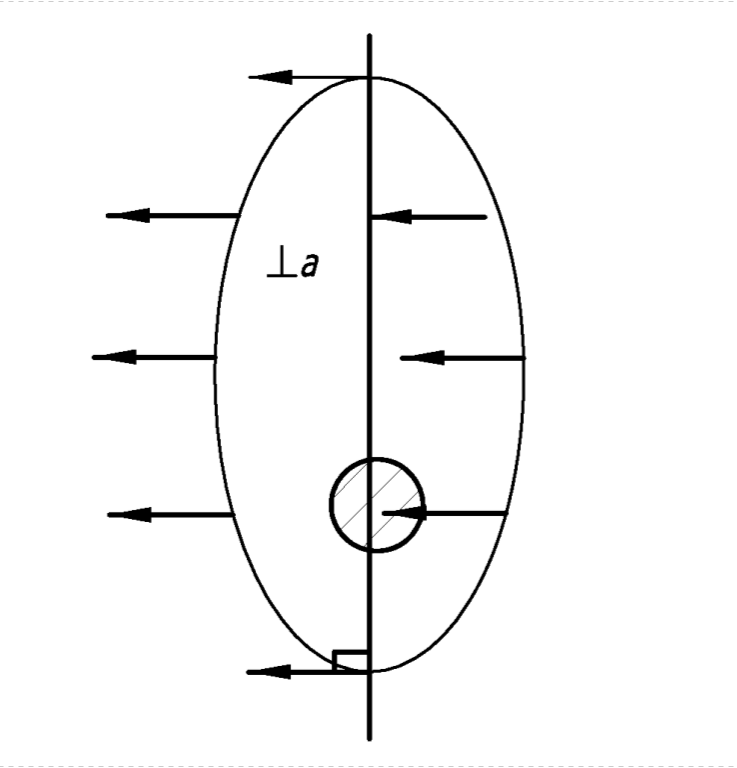
\includegraphics[width=0.5\textwidth]{figures/fixed-perpendicular.png}
  \caption{Steering law perpendicular to the semimajor axis.}
  \label{fig:perpendicular}
\end{figure}

Using a geometrical reasoning, it is straightforward to see that the condition for applying thrust in a direction that is orthogonal to the semimajor axis of the orbit is $f_r = f \sin{\ta}$ and $f_{\ta} = f \cos{\ta}$. However, this approach can lead to numerical instabilities when the eccentricity is low and the semimajor axis itself is ill-defined. In our implementation we opted for fixing the thrust direction $\vec{a}_d = f \vec{\hat{p}}$ at the beginning of the integration: %using the initial position vector when $e < 0.001$.

\[ \vec{\hat{p}} = \begin{cases}
\vec{e} / e   & \text{if } e > 0.001 \\
\vec{r}_0 / r & \text{otherwise}
\end{cases}
\]

where $\vec{e}$ is the eccentricity vector.

To validate this guidance law we have employed an example found in \cite{ruggiero2011low} consisting in the disposal of a Sun-synchronous orbit by increasing its eccentricity, described in table~\ref{tab:sso}. Notice that some values are not explicitly written in the paper and we had to infer them from the results.

\begin{table}
\centering
\begin{tabular}{|l|l|}
\hline
\textbf{Attractor}            & Earth \\ \hline
\textbf{Specific thrust}            & $2.4 \cdot 10^{-7}$ km/s\textsuperscript{2}      \\ \hline
\textbf{Altitude}                   & $900$ km                                   \\ \hline
\textbf{Initial eccentricity $e_0$} & $0$                                        \\ \hline
\textbf{Final eccentricity $e_f$}   & $0.1245$ (reverse-engineered from results) \\ \hline
\textbf{Time of flight $t_f$}   & $29.697$ days (reverse-engineered from results) \\ \hline
\textbf{Cost $\Delta V$}   & $0.6158$ km/s \\ \hline
\end{tabular}
\caption{Disposal of a Sun-synchronous orbit from \cite{ruggiero2011low}.}
\label{tab:sso}
\end{table}

On the other hand, although it is not mentioned in the original paper, a change of sign is needed depending on the sign of $e_f - e_0$, so we tested the reverse case as well using the same data.

\subsection{Argument of periapsis adjustment}

According to \cite{pollard1998evaluation}, we can adjust the argument of periapsis $\omega$ while holding the semimajor axis $a$ and the eccentricity $e$ constant by applying thrust along a direction that is parallel to the semimajor axis of the orbit. The resulting secular rate of change of $\omega$ is:

\[
\secular{\deriv{\omega}{t}} = \mp \frac{3}{2} f \sqrt{\frac{a}{\mu}} \frac{\sqrt{1 - e^2}}{e} + \dot{\omega}
\]

where again we are not considering the possibility of discontinuous thrust and $\dot{\omega}$ is the natural apsidal rotation due to a the oblateness of the attractor. For the case of the Earth, this would be \cite{vallado2001fundamentals}:

\[
\dot{\omega} = \frac{3 n R_{\Earth}^2 J_2}{4 a^2 (1 - e^2)^2} (4 - 5 \sin^2 i)
\]

where $n$ is the mean motion and $J_2 = 1.08262668 \cdot 10^{-3}$ is the second degree harmonic. The required $\Delta V$ considering the apsidal rotation is:

\begin{equation}
\Delta V = \frac{\Delta \omega}{\frac{3}{2} \sign{(\Delta \omega)} \sqrt{\frac{a}{\mu}} \frac{\sqrt{1 - e^2}}{e} + \frac{\dot{\omega}}{f}}
\label{eq:dvargp}
\end{equation}

To validate this steering law we have taken another example from \cite{ruggiero2011low}, in this case the periapsis correction of a standard Soyuz geostationary transfer orbit (GTO) summarized in table~\ref{tab:gto}. The shape of the orbit has been taken from the Soyuz Users Manual, issue 2 revision 0.

The example of Ruggiero does not take into account the natural apsidal rotation, and so the question opens whether this is a sensible choice or not. Looking at the denominator of equation~\ref{eq:dvargp}, we are therefore interested in comparing $\dot{\omega} / f$ with the rest. Dimensional analysis yields:

\[
\frac{\frac{\dot{\omega}}{f}}{\frac{3}{2} \sign (\Delta \omega) \sqrt{\frac{a}{\mu}} \frac{\sqrt{1 - e^2}}{e}} \sim %
\frac{\frac{\dot{\omega}}{f}}{\frac{1}{V}} \sim %
V \frac{\dot{\omega}}{f} \sim %
\frac{\mu R_{\Earth}^2 J_2}{a^4 f} \approx \frac{1}{5}
\]

Notice that in this case $\sqrt{1 - e^2} \sim e$. The natural apsidal rotation is by no means negligible with respect to the action of the thrust, but we will accept not taking it into account in the absence of better numerical validation examples.

\begin{table}
\centering
\begin{tabular}{|l|l|}
\hline
\textbf{Attractor}            & Earth \\ \hline
\textbf{Specific thrust}            & $2.4 \cdot 10^{-7}$ km/s\textsuperscript{2}      \\ \hline
\textbf{Altitude of apoapsis $r_a - R_{\Earth}$} & $35950$ km \\ \hline
\textbf{Altitude of periapsis $r_p - R_{\Earth}$} & $250$ km \\ \hline
\textbf{Initial argument of periapsis $\omega_0$} & $178$ deg \\ \hline
\textbf{Argument of periapsis change $\Delta \omega_0$} & $5$ deg \\ \hline
\textbf{Time of flight $t_f$} & $12$ days (approximate) \\ \hline
\textbf{Cost $\Delta V$} & $0.2489$ km/s \\ \hline
\end{tabular}
\caption{Periapsis correction of a standard Soyuz geostationary transfer orbit from \cite{ruggiero2011low}.}
\label{tab:gto}
\end{table}

\section{Non planar maneuvers} \label{sec:metnonplanar}

We now study maneuvers that affect the orbital elements which define the plane of the orbit as well as the rest, specifically the inclination $i$. Although there are some guidance laws to modify $\Omega$ available in the literature (see \cite{kechichian2010analytic,pollard1997simplified}), we have not considered them in this work because, on the one hand, the $(a_0, \Omega_0) \rightarrow (a_f, \Omega_0), e = 0$ proposed by Kéchichian can be treated in the same way as the $(a_0, i_0) \rightarrow (a_f, i_0), e = 0$ studied in section~\ref{sec:metedelbaum} and, on the other hand, Pollard suggests that taking advantage of the natural nodal regression and its dependence on altitude is preferred.

The advantage of using combined maneuvers is evident when we consider the required increment of velocity for an inclination change of a circular orbit using an impulsive maneuver \cite{vallado2001fundamentals}:

\[
\Delta V = 2 V_0 \sin \frac{\Delta i}{2}
\]

For moderate values of $\Delta i$, the required $\Delta V$ can be of the same order of the velocity itself, which is usually in the range of tenths of kilometers per second for low Earth orbits. It is therefore an extremely expensive maneuver that is better performed at large distances of the attractor, where the velocity decreases. In the following sections we will therefore study two steering programs that combine a change in inclination with another orbital element.

\subsection{Combined semimajor axis and inclination change} \label{sec:metedelbaum}

Among other results, and as previously mentioned, \cite{edelbaum1961propulsion} presented an extremely interesting guidance law for a combined change of semimajor axis and inclination, which was later reformulated in \cite{kechichian1997reformulation} to simplify the algorithms involved and potential software implementations. We comment here the most salient part of the derivation.

The thrust is applied along the tangential and out of plane components, resulting $f_T = f \cos{\beta}$ and $f_h = f \sin{\beta}$ where $\beta$, called the thrust yaw angle, will be the control parameter. If $\beta$ is held constant during each revolution (hence piecewise constant) and we switch the sign at the orbital antinodes, the only orbital elements that will experiment secular variation will be $a$ and $i$. Averaging out the orbital position $\ta$ transforms $\beta$ in a continuous function of time, resulting in the following equations of motion:

\begin{align*}
\secular{\deriv{i}{t}} & = \frac{2 f \sin{\beta}}{\pi V} \\
\secular{\deriv{V}{t}} & = -f \cos{\beta}
\end{align*}

Here Kéchichian departs from Edelbaum and casts these equations as a minimum time transfer problem between initial and final $i$ and $V$. After applying techniques from the calculus of variations, he arrives to the control law

\[
\tan{\beta(t)} = \frac{V_0 \sin{\beta_0}}{V_0 \cos{\beta_0} - f \cdot t}
\]

in terms of time $t$ and the parameters of the problem, where

\[
\tan{\beta_0} = \frac{\sin{ \left( \frac{\pi}{2} \Delta i \right)}}{\frac{V_0}{V} - \cos{ \left( \frac{\pi}{2} \Delta i \right)}}
\]

Both quantities can be easily computed without ambiguity by using appropriate \verb|arctan2| routines. The time history of both the velocity and the relative inclination are also known:

\[
V = \sqrt{ V_0^2 - 2 V_0 f \cdot t \cos{\beta_0} + f^2 t^2 }
\]
\[
i - i_0 = \frac{2}{\pi} \left( \arctan{\left( \frac{f \cdot t - V_0 \cos{\beta_0}}{V_0 \sin{\beta_0}}\right)} + \frac{\pi}{2} - \beta_0 \right)
\]

As will be seen graphically in the next chapter, the orbit smoothly gets larger to reduce the velocity and perform most of the inclination change far away from the attractor and then shrinks back to the required final semimajor axis. We note that for $\Delta i = 2~\text{rad} = 114.59~\text{deg}$ both $\beta_0$ and $\beta$ become zero: this represents the limit case when the spacecraft reaches infinity and then the inclination change is performed at no cost. In this case, continuous thrust is no longer advantageous and a bitangent impulsive maneuver is preferred.

To validate this guidance law we used two LEO to GEO examples explained in great detail in \cite{kechichian1997reformulation} and summarized in table~\ref{tab:leogeo}.

\begin{table}[b]
\centering
\begin{tabular}{|l|l|}
\hline
\textbf{Attractor} & Earth \\ \hline
\textbf{Specific thrust} & $3.5 \cdot 10^{-7}$ km/s\textsuperscript{2} \\ \hline
\textbf{Initial semimajor axis $a_0$} & $7\,000$ km \\ \hline
\textbf{Final semimajor axis $a_f$} & $42\,166$ km \\ \hline
\textbf{Initial inclination $i_0$} & $28.5$ deg and $90$ deg \\ \hline
\textbf{Final inclination $i_f$} & $0$ deg \\ \hline
\textbf{Time of flight $t_f$} & $191.26295$ days and $335$ days \\ \hline
\textbf{Cost $\Delta V$} & $5.78378$ km/s and $10.13$ km/s \\ \hline
\end{tabular}
\caption{LEO to GEO transfers from \cite{kechichian1997reformulation}.}
\label{tab:leogeo}
\end{table}

\subsection{Combined eccentricity and inclination change}

Following previous works in the topic, \cite{pollard2000simplified} presented several continuous thrust strategies, in particular a control law for a combined eccentricity and inclination change. Instead of deriving an optimal steering program, Pollard studies how applying an in-plane acceleration perpendicular to the semimajor axis of the orbit with the intent of changing the eccentricity affects in turn the inclination, and adjusts the yaw angle so the final eccentricity and inclination requirements are met at the same time. In this case, the secular variation of eccentricity will be

\begin{table}[b]
\centering
\begin{tabular}{|l|c|c|c|c|c|}
\hline
                                    & Case 1   & Case 2   & Case 3   & Case 4        & Case 5        \\ \hline
\textbf{Attractor}                  & \multicolumn{5}{c|}{Earth}                                     \\ \hline
\textbf{Specific thrust}            & \multicolumn{5}{c|}{$2.4 \cdot 10^{-7}$ km/s2}                 \\ \hline
\textbf{Semimajor axis $a$}         & \multicolumn{5}{c|}{$42\,164$ km}                              \\ \hline
\textbf{Initial eccentricity $e_0$} & $0.1$    & $0.2$    & $0.4$    & $0.6$         & $0.8$         \\ \hline
%\textbf{Final eccentricity $e_f$}   & \multicolumn{5}{c|}{$0$}                                       \\ \hline
%\textbf{Initial inclination $i_0$}  & \multicolumn{5}{c|}{$0$ deg}                                   \\ \hline
\textbf{Final inclination $i_f$}    & \multicolumn{3}{c|}{$20$ deg}  & \multicolumn{2}{c|}{$16$ deg} \\ \hline
\textbf{Yaw angle $\beta$ (deg)}    & $83.043$ & $76.087$ & $61.522$ & $40$          & $16.304$      \\ \hline
\textbf{Cost $\Delta V$ (km/s)}     & $1.6789$ & $1.6890$ & $1.7592$ & $1.7241$      & $1.9799$      \\ \hline
\end{tabular}
\caption{Cases extracted from \cite{pollard2000simplified}.}
\label{tab:geoinc}
\end{table}

\[
\left| \secular{\deriv{e}{t}} \right| = \frac{3}{2} f \cos{\left| \beta \right|} \sqrt{\frac{a}{\mu}} \sqrt{1 - e^2}
\]

where $\beta$ is again the yaw angle. Notice that setting $\beta = 0$ recovers the case studied in section~\ref{sec:metecc}. Under the assumption that the sign of the yaw angle reverses at minor axis crossings, the secular rate of change of the inclination will be

\[
\left| \secular{\deriv{i}{t}} \right| = \frac{f \sin{\left| \beta \right|}}{\pi} \sqrt{\frac{a}{\mu}} \left| \cos{\omega} \right| \frac{2 (1 + e^2)}{\sqrt{1 - e^2}}
\]

Note that the inclination change will be more efficient when $\left| \cos{\omega} \right|$ approaches 1, that is, $\omega \approx 0~\text{deg}$ or $\omega \approx 180~\text{deg}$. Dividing these two rates of change and integrating assuming $\omega$ constant yields the control law \cite{pollard2000simplified}:

\[
\tan{\left| \beta \right|} = \left| \frac{3 \pi (i_f - i_0)}{4 \cos{\omega} \left( \log{\left(\frac{e_f + 1}{e_0 + 1} \frac{e_0 - 1}{e_f - 1}\right)} - e_f + e_0 \right)} \right|
\]

The required $\Delta V$ for this case will be:

\[
\Delta V = \frac{2}{3} \circvel{a} \frac{\left| \arcsin{e_0} - \arcsin{e_f} \right|}{\cos{\left| \beta \right|}}
\]

Since no numerical validation cases are explicitly given for this guidance law, we have extracted five data points from the plots of the original paper using an online software\footnote{\url{http://arohatgi.info/WebPlotDigitizer/app/}}. All five have been used for the analytical validation and only one (and its reverse) for the numerical validation. The cases are summarized in table~\ref{tab:geoinc}.
